\chapter{Declarative Geometry Constraint Solver}
\label{chap:declarative}

\section{Overview}

The third module is a declarative geometry constraint solver. Given a
user-specified topology of a diagram and various constraints on
segments and angles, this module attempts to solve the specification
by instantiating a figure that satisfies the constraints.

The solver is implemented using propagators, uses new types of partial
information about point regions and direction intervals, and focuses
on emulating the mental process of building and solving constrained
figures in the mind's eye. The physical nature of this process is
captured by forming analogies between geometry diagrams and mechanical
linkages of bars and joints.

After providing a brief overview of the mechanical analogies and quick
background on the propagator system, I examine an example of the
system solving a set of constraints for an under-constrained
rectangle. Then, I describe the module implementation, starting with
the new partial information representations and linkage constraints
before explaining how mechanisms are assembled and solved. Finally,
some limitations and extensions are discussed.

%% Outline
%% - Mechanical Analogies
%% - Propagator System
%% - Partial Information Structures
%% - Linkages
%% - Building a Mechanism
%% - Solving a Mechanism
%% - Discussion

\subsection{Mechanical Analogies}

Mechanical analogies are often applied to mathematical problems to
yield alternate, often more-intuitive solutions. Several texts such as
\cite{levi2009mathematical} and \cite{uspenskii1961some} explore this
and provide examples such as deriving the Pythagorean Theorem from a
physical example dealing with water pressure in and torque on a
rotating drum.

In this system, mechanical analogies are used to represent the physics
simulation going on as one mentally manipulates a diagram ``in the
mind's eye''. Often, given a diagram with constraints, one can imagine
assembling a physical example of the figure out of bars and joints in
one's head.  Some bars can be sliding to make their lengths adjustable
whereas others are constrained to be of equal length.  As a person
moves and wiggles these pieces to assemble satisfying mechanisms, they
can examine whether the resulting mechanisms retain properties across
instances and generalize such invariants into theorems.

This module simulates this process by assembling mechanisms of bars
and joints, and using a propagator system to simulate incrementally
selecting where bars and joints are positioned while maintaining local
physical constraints.

\subsection{Propagator System}

The declarative geometry solver is built upon an existing propagator
system created by Alexey Radul under the advisement of Gerald Jay
Sussman \cite{gjs-propagator}. The propagator system allows a user to
create cells and connect them with propagator constraints. As content
is added to cells, their neighbors are notified and updated with
computations performed on the new information. Often, cells maintain a
representation of partial information about their content and merge
new information from several sources.

This module uses Radul's propagation system to handle the underlying
propagation of data, but implements constraints, partial information
types, specification protocols, and input formats particular to geometric
figures.

\section{Example of Solving Geometric Constraints}
\label{sec:example-solving}

I begin by fully explaining an example. The geometry problem of
inadequately constrained rectangles was introduced in the first
example of Chapter~\ref{chap:motivation} on page
\pageref{example-1}. The second proposed set of constraints in that
problem was expressed as a mechanism in Example~\ref{is-rect-2} in the
demonstration (page \pageref{is-rect-2}), and is repeated here in
Example~\ref{is-rect-specs}. Example~\ref{is-rect-solved} shows the
module's print messages as it solves the mechanism.

The illustrations in Explanation~\ref{illustration} and accompanying text
on the following pages explain how propagation is used to solve this
mechanism.

\begin{code-example}
[label=is-rect-specs]
{Rectangle Constraints Example}
(define (is-this-a-rectangle-2)
  (m:mechanism
   (m:establish-polygon-topology 'a 'b 'c 'd)
   (m:c-length-equal (m:bar 'a 'd) (m:bar 'b 'c))
   (m:c-right-angle (m:joint 'd))
   (m:c-angle-equal (m:joint 'a) (m:joint 'c))))
\end{code-example}

\begin{img-example}
[label=is-rect-solved]
{Solved Constraints}{images/rect-demo-2.png}
=> (m:run-mechanism (is-this-a-rectangle-2))

(specifying-bar m:bar:d:a .6742252545577186)
(initializing-direction m:bar:d:a-dir (direction 4.382829365403101))
(initializing-point m:bar:d:a-p1 (0 0))
(specifying-joint m:joint:c:b:a 2.65583669872538)
\end{img-example}

Solving a mechanism involves repeatedly selecting positions, lengths,
angles, and directions that are not fully specified and selecting
values within the domain of that element's current partial
information. As values are specified, the wiring of the propagator
model propagates further partial information to other values.

\refstepcounter{tcb@cnt@code-example}\label{illustration}
\begin{figure}[h]
\captionsetup{labelformat=empty}
\caption{{\bf Propagation Explanation
    \arabic{chapter}.\arabic{tcb@cnt@code-example}:} This series of
  illustrations depicts the propagation steps that occur to enable the
  system to solve the underconstrained rectangle from
  Example~\ref{is-rect-specs}.
}
\centering
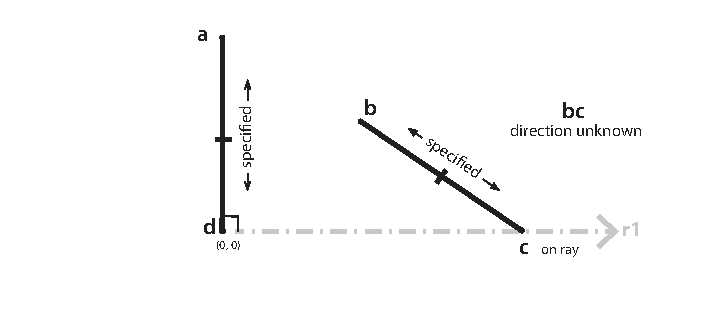
\includegraphics[width=.95\textwidth]{diagrams/is-rect-explained-boards-1.eps}
\caption{{\bf Step 1:} The first value the module specifies is the
  length of bar \texttt{ad}. In doing so, it also initializes the
  bar's endpoint and direction to anchor it on the canvas. Because
  joint \texttt{d} is constrained to be a right angle, the system knows
  the direction but not length of bar \texttt{dc}. It propagates the
  partial information that point \texttt{c} is on the ray $r1$ extending
  out from \texttt{d} to the cell within point
  \texttt{c}. Furthermore, since bars \texttt{ad} and \texttt{bc} are
  constrained to have equal length, at this point, bar \texttt{bc} also knows
  its length but not direction. Next, the system specifies joint angle \texttt{b}:}
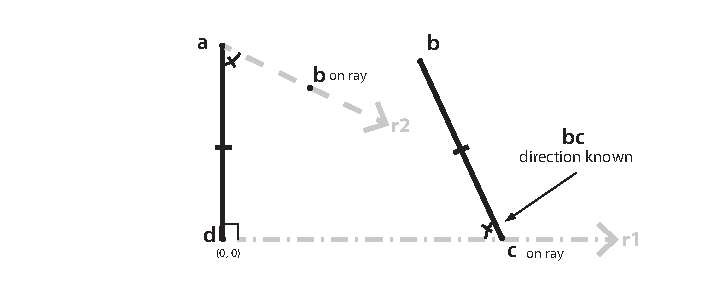
\includegraphics[width=.95\textwidth]{diagrams/is-rect-explained-boards-2.eps}
\caption{{\bf Step 2:} Once the angle measure of \texttt{b} is
  specified, constraints using the sum of angles in the specified
  polygon and a ``slice'' constraint on the pair of constrained angles
  will set the angle measures of joints \texttt{a} and \texttt{c} to
  be half of the remaining total:
  $\text{\texttt{a,c}}\protect\leftarrow\frac{2\protect\pi -
    \text{\texttt{b}} - \text{\texttt{d}}}{2}$. With these angles
  specified, point \texttt{b} is informed that it is on the ray $r2$
  and bar \texttt{bc} now knows both its length and direction.}
\vspace{-10em}
\end{figure}

\newpage
\begin{figure}[h]
\captionsetup{labelformat=empty}
\caption{{\bf Propagation Explanation
    \arabic{chapter}.\arabic{tcb@cnt@code-example} continued:} This series of
  illustrations depicts the propagation steps that occur to enable the
  system to solve the underconstrained rectangle solved in
  Example~\ref{is-rect-specs}.}
\centering
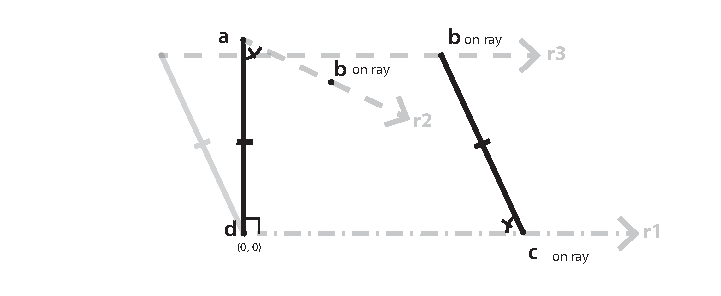
\includegraphics[width=.95\textwidth]{diagrams/is-rect-explained-boards-3.eps}
\caption{{\bf Step 3:} Since now both the length and direction of bar
  \texttt{bc} are known and point \texttt{c} is known to be on ray
  $r1$, the propagation constraints can translate this ray by the
  length and direction of \texttt{bc} and provide the information that
  point \texttt{b} must therefore also be on ray $r3$. This emulates
  the physical process of sliding bar \texttt{bc} along ray $r1$.}
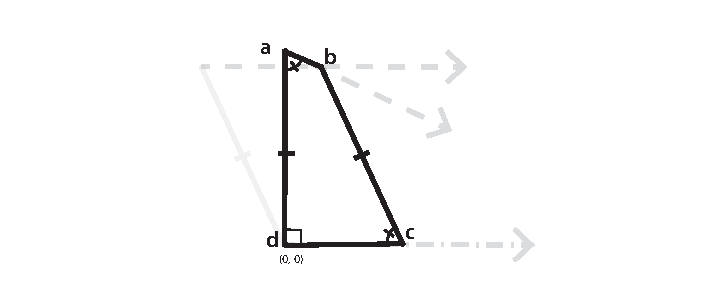
\includegraphics[width=.95\textwidth]{diagrams/is-rect-explained-boards-4.eps}
\caption{{\bf Step 4:} The information about point \texttt{b} being on
  rays $r2$ and $r3$ is merged via ray intersection to fully determine
  the location of \texttt{b}. Then, once point \texttt{b} is
  specified, since the length and direction of bar \texttt{bc} is
  known, propagation sets the value and location of point \texttt{c},
  yielding a fully-specified solution.}
\vspace{-1.5em}
\end{figure}
Similar steps allow propagation to solve specifications for many
figures including isosceles triangles, parallelograms, and
quadrilaterals from their diagonals. Several of these are shown in
Section \ref{demo:sec:declarative}. In cases when bars have their
length and one endpoint determined first, the propagators specify that
the other endpoint is on an arc of a circle. The next sections
describe the implementation of these partial information structures
before explaining bar and joint structures and how mechanisms are
built and solved.

\newpage
\section{Partial Information Structures}

Radul's propagation system typically used numeric intervals for
partial information. The declarative constraint solver uses some
standard numeric intervals, but also uses its own module-specific
partial information structures. These include \texttt{regions} and
\texttt{direction-intervals}, described below:

\subsection{Regions}

Regions are the partial information structure for point locations and
represent subsets of the plane where the points could be
located. These could be arbitrarily complex regions of the plane, but
the module currently implements point sets, rays, and arcs as shown in
Listing~\ref{regions}. As new information about locations are
provided, regions are merged by intersection. A contradiction region
represents an empty region.

\enlargethispage*{\baselineskip}
\begin{code-listing}
[label=regions]
{Region Structures}
(define-record-type <m:point-set>
  (%m:make-point-set points) ...)

(define-record-type <m:ray>
  (%m:make-ray endpoint direction) ...)

(define-record-type <m:arc>
  (m:make-arc center-point radius dir-interval) ...)

(define-record-type <m:region-contradiction>
  (m:make-region-contradiction error-regions) ...)

(defhandler merge m:intersect-regions m:region? m:region?)
\end{code-listing}

\subsection{Direction Intervals}

In addition, a module-specific direction interval structure is used
for the partial information about directions. Several additional
utilities were needed for working with and merging direction intervals
since directions form a periodic range $[0,2\pi)$. Currently, the
  subsystem treats an intersection of direction intervals that would
  yield multiple distinct direction intervals as providing no
  new information.

\section{Bar and Joint Constraints}

The solver uses bar and joint linkages to represent segments and
angles. These structures are composed of propagator cells storing
information about locations, lengths, directions, and angles. To
assist with some of the propagation between these cells, the module
uses substructures for points and vectors.

Point structures contain both numeric Cartesian coordinate cells and a cell
containing region structures. The propagators \texttt{m:x-y->region}
and \texttt{m:region->x,y} transform location information between
these representations.

\begin{code-listing}
[label=point-region]
{Points and Regions}
(define (m:make-point)
  (let-cells (x y region)
    (p:m:x-y->region x y region)
    (p:m:region->x region x)
    (p:m:region->y region y)
    (%m:make-point x y region)))

(define (m:x-y->region x y)
  (m:make-singular-point-set (make-point x y)))
(propagatify m:x-y->region)

(define (m:region->x region)
  (if (m:singular-point-set? region)
      (point-x (m:singular-point-set-point region))
      nothing))
(propagatify m:region->x)
\end{code-listing}

Vectors represent the difference between two points and bidirectionally
constrain both rectangular and polar information.

\begin{code-listing}
[label=vec-struct]
{Vectors}
(define (m:make-vec)
  (let-cells (dx dy length direction)
    (p:make-direction (e:atan2 dy dx) direction)
    (p:sqrt (e:+ (e:square dx)
                 (e:square dy))
            length)
    (p:* length (e:direction-cos direction) dx)
    (p:* length (e:direction-sin direction) dy)
    (%m:make-vec dx dy length direction)))
\end{code-listing}

\subsection{Bar Structure and Constraints}

As seen in Listing~\ref{bar-struct}, bar structure contains two
\texttt{m:point}s and a \texttt{m:vec} representing the distance and
direction between the points. The bar links these structures together
using simple bidirectional constraints on the coordinates. These
constrains will only propagate information when the bar's length and
direction are fully specified. \texttt{m:p1->p2-bar-propagator} and
its reverse handle the other cases.

\begin{code-listing}
[label=bar-struct]
{Basic Bar Structure}
(define (m:make-bar bar-id)
  (let ((p1 (m:make-point))
        (p2 (m:make-point))
        (v (m:make-vec)))
    (c:+ (m:point-x p1) (m:vec-dx v)
         (m:point-x p2))
    (c:+ (m:point-y p1) (m:vec-dy v)
         (m:point-y p2))
    (let ((bar (%m:make-bar p1 p2 v)))
      (m:p1->p2-bar-propagator p1 p2 bar)
      (m:p2->p1-bar-propagator p2 p1 bar)
      bar)))
\end{code-listing}

The propagators specified by \texttt{m:p1->p2-bar-propagator} shown in
Listing~\ref{bar-propagator} propagate partial information about point
locations based on whether the bar's direction or length is
determined. \texttt{m:x-y-length-di->region} handles the case where
only the length of the bar is specifies and adds information to the
other endpoint's region cell that it is on the arc formed from the
bar's length and current direction interval. This implementation is
seen in Listing \ref{bar-propagator}.

\begin{code-listing}
[label=bar-propagator]
{Bar Region Propagator}
(define (m:p1->p2-bar-propagator p1 p2 bar)
  (let ((p1x (m:point-x p1))
        (p1y (m:point-y p1))
        (p1r (m:point-region p1))
        (p2r (m:point-region p2))
        (length (m:bar-length bar))
        (dir (m:bar-direction bar)))
    (p:m:x-y-direction->region p1x p1y dir p2r)
    (p:m:x-y-length-di->region p1x p1y length dir p2r)
    (p:m:region-length-direction->region p1r length dir p2r)))
(define (m:x-y-length-di->region px py length dir-interval)
  (if (direction-interval? dir-interval)
      (let ((vertex (make-point px py)))
        (m:make-arc vertex length dir-interval))
      nothing))
\end{code-listing}
\vspace{-1em}
\subsection{Joint Structure and Constraints}

Joints are represented by a vertex point, two directions, and an angle
representing the measure between the directions. Propagators
bidirectionally constrain the angle measure to reflect and update the
ranges of the joint's directions.  Special mechanism-specific
operators adding and subtracting directions were created since both
the direction and angle argument could be intervals. Creating a joint
also initializes its measure to the range $[0, \pi]$, reflecting the
maximum angle sweep.

\begin{code-listing}
{Joint Constraints}
(define (m:make-joint)
  (let ((vertex (m:make-point)))
    (let-cells (dir-1 dir-2 theta)
      (p:m:add-to-direction dir-1 theta dir-2)
      (p:m:add-to-direction dir-2 (e:negate theta) dir-1)
      (p:m:subtract-directions dir-2 dir-1 theta)
      (m:instantiate theta (make-interval 0 *max-joint-swing*) 'theta)
      (%m:make-joint vertex dir-1 dir-2 theta))))
\end{code-listing}

\enlargethispage*{\baselineskip}
\vspace{-1em}
\section{User-specified Constraints}

In addition to constraints resulting from the bar and joint
connections, users can specify additional constraints on the
mechanism. Listing~\ref{constraint-struct} shows the structure for a
user constraint. These structures include a name, a list of bar or
joint identifiers the constraint constrains, and a procedure used to
apply the constraint.

\begin{code-listing}
[label=constraint-struct]
{User Constraints}
(define-record-type <m:constraint>
  (m:make-constraint type args constraint-procedure) ...)
\end{code-listing}
\begin{code-listing}
[label=bar-eq]
{Bar Length Equality}
(define (m:c-length-equal bar-id-1 bar-id-2)
  (m:make-constraint
   'm:c-length-equal
   (list bar-id-1 bar-id-2)
   (lambda (m)
     (let ((bar-1 (m:lookup m bar-id-1))
           (bar-2 (m:lookup m bar-id-2)))
       (c:id (m:bar-length bar-1)
             (m:bar-length bar-2))))))
\end{code-listing}

This constraint procedure takes the assembled mechanism as its
argument. As shown in Listing~\ref{bar-eq}, such procedures
typically look up mechanism elements by bar or joint identifiers and
introduce additional constraints. In \texttt{m:c-length-equal}, the
lengths of the two bars are set to be identical to one another.

\subsection{Slice Constraints}

In addition to general user constraints, mechanisms are also support
slice constraints. These slices are structured in the same manner as
constraints but are applied after all other user constraints, and thus
can use information about user constraints in adding their
propagators. In particular, the system uses slices to determine the
values of cells that are constrained as equal to one another within a
sum, once the total of the sum and all other cells in the sum have
been determined. This process is inspired by Gerald Jay Sussman's use
of slices to represent local patterns and help determine values in
propagation networks for circuit design \cite{gjs-slices}.

\section{Assembling Mechanisms}
\enlargethispage*{\baselineskip}

Mechanism structures in the declarative system are the analogs of
figures from the imperative system.  Here, instead of grouping
geometry elements, the mechanism group linkages and constraints. As
seen in Listing~\ref{mechanism-struct}, \texttt{m:mechanism} will
flatten and separate its arguments. Then, in addition to storing the
components in a record structure, \texttt{m:make-mechanism} will also
build hash tables for looking up bars and joints by their endpoint and
vertex names.

\begin{code-listing}
[label=mechanism-struct]
{Mechanism Structure}
(define-record-type <m:mechanism>
    (%m:make-mechanism bars joints constraints slices
                        bar-table joint-table joint-by-vertex-table)...)

(define (m:mechanism . args)
  (let ((elements (flatten args)))
    (let ((bars (m:dedupe-bars (filter m:bar? elements)))
          (joints (filter m:joint? elements))
          (constraints (filter m:constraint? elements))
          (slices (filter m:slice? elements)))
      (m:make-mechanism bars joints constraints slices))))
\end{code-listing}

To assist with specifying the bars and joints for a closed polygon,
the utility \texttt{m:establish-polygon-topology} is often used. The
procedure takes $n$ vertex names as its arguments and returns $n$ bars
and $n$ joints. It uses the linkage constructors
\texttt{m:make-named-*} to attach names to the structures.  Such names
are later used to attach linkages to one another and to lookup
elements in constraint procedures.

\begin{code-listing}
[label=est-topo]
{Establishing Topology}
(define (m:establish-polygon-topology . point-names)
  (if (< (length point-names) 3)
      (error "Min polygon size: 3"))
  (let ((extended-point-names
         (append point-names (list (car point-names) (cadr point-names)))))
    (let ((bars (map (lambda (p1-name p2-name)
                       (m:make-named-bar p1-name p2-name))
                     point-names (cdr extended-point-names)))
          (joints (map (lambda (p1-name vertex-name p2-name)
                         (m:make-named-joint p1-name vertex-name p2-name))
                       (cddr extended-point-names)
                       (cdr extended-point-names)
                       point-names)))
      (append bars joints
              (list (m:polygon-sum-slice (map m:joint-name joints)))))))
\end{code-listing}

Once specified, mechanisms can be assembled using
\texttt{m:build-mechanism}.  That procedure first identifies all joint
vertices with the same names as being identical to one another to
handle topologies in which multiple joints share vertices. Then it
assembles bars and joints based on their names.

\begin{code-listing}
{Building Mechanisms}
(define (m:build-mechanism m)
  (m:identify-vertices m)
  (m:assemble-linkages (m:mechanism-bars m)
                       (m:mechanism-joints m))
  (m:apply-mechanism-constraints m)
  (m:apply-slices m))
\end{code-listing}

When assembling the mechanism, bars are identified into or out of the
arms of joints that share their names. Joints names refer to the three
vertices they connect and bar names refer to their two endpoint
vertices.  \texttt{m:identify-into-arm-1} (\ref{identifying-points})
demonstrates how bars and joints get attached to one
another. Corresponding point locations and directions are constrained
to be identical to one another via \texttt{c:id}. Identifying two
points involves identifying all of its component properties.

\begin{code-listing}
[label=identifying-points]
{Identifying points}
(define (m:identify-into-arm-1 joint bar)
  (m:set-joint-arm-1 joint bar)
  (m:identify-points (m:joint-vertex joint) (m:bar-p2 bar))
  (c:id (ce:reverse-direction (m:joint-dir-1 joint))
        (m:bar-direction bar)))

(define (m:identify-points p1 p2)
  (for-each (lambda (getter)
              (c:id (getter p1) (getter p2)))
            (list m:point-x m:point-y m:point-region)))
\end{code-listing}

\section{Solving Mechanisms}

Once assembled, mechanisms can be solved via
\texttt{m:solve-mechanism}. Solving a mechanism involves repeatedly
selecting position, lengths, angles, and directions that are not fully
specified and selecting values within the domain of that element's
current partial information structure. As values are specified, the
constraint wiring of the propagator model propagates updated partial
information to other values.


\begin{code-listing}
[label=solve-mechanism]
{Solving Mechanisms}
(define (m:solve-mechanism m)
  (m:initialize-solve)
  (let lp ()
    (run)
    (cond ((m:mechanism-contradictory? m)
           (m:draw-mechanism m c)
           #f)
          ((not (m:mechanism-fully-specified? m))
           (if (m:specify-something m)
               (lp)
               (error "Couldn't find anything to specify.")))
          (else 'mechanism-built))))
\end{code-listing}

The ordering of what is specified is guided by a heuristic in
\texttt{m:specify-something} (\ref{specify-something}). This heuristic
was determined empirically and helps the majority of the examples I
explored converge to solutions. It generally prefers specifying the
most constrained values first. However, in some scenarios, specifying
values in the wrong order can yield premature
contradictions. Additionally, sometimes partial information about a
value is incomplete and picking a value arbitrarily may fail. A
planned extension will attempt to recover from such situations more
gracefully by trying other values or orderings for specifying
components.

\begin{code-listing}
[label=specify-something]
{Specifying and Instantiating Values}
(define (m:specify-something m)
  (or
   (m:specify-bar-if m m:constrained?)
   (m:specify-joint-if m m:constrained?)
   (m:specify-joint-if m m:joint-anchored-and-arm-lengths-specified?)
   (m:initialize-bar-if m m:bar-length-specified?)
   ...)
\end{code-listing}

The system uses \texttt{m:instantiate} to add content to cells. As
seen in Listing~\ref{instantiate}, \texttt{m:instantiate} wraps
the value in a truth maintenance system structure provided by Radul's
propagator system. These structures maintain dependencies for values, can report
which sets of premises are at odds with one another and allow
individual choices to be removed and replaced with new values.
\enlargethispage*{\baselineskip}

\begin{code-listing}
[label=instantiate]
{Instantiating Values with TMS}
(define (m:instantiate cell value premise)
  (add-content cell (make-tms (contingent value (list premise)))))
\end{code-listing}

\subsection{Interfacing with imperative diagrams}

Finally, as shown in Listing~\ref{to-figure},
\texttt{m:mechanism->figure} can convert fully specified mechanisms
into their corresponding figures so they can be observed and analyzed.

\begin{code-listing}
[label=to-figure]
{Converting to Figure}
(define (m:mechanism->figure m)
  (let ((points (map m:joint->figure-point (m:mechanism-joints m)))
        (segments (map m:bar->figure-segment (m:mechanism-bars m)))
        (angles (map m:joint->figure-angle (m:mechanism-joints m))))
    (apply figure (filter identity (append points segments angles)))))
\end{code-listing}

\section{Discussion and Extensions}

The process of incrementally specifying values and propagating
properties implied by constraints is able to solve many geometry
constraint problems. Radul's propagator network framework helps with
propagating local constraints, representing partial information, and
merging updates.

Although the module successfully solves many useful mechanism
configurations, adding propagation alone is not a magic wand. Even
with selecting values based on updated partial information and
heuristics for choosing items to specify, there are several instances
in which the module can fail to solve a mechanism specification that
actually has a solution. Because of such false negatives, the
constraint solver is never able to report that a set of constraints is
infeasible, just that it hasn't been able to produce a solution. This
works for my main use cases as the module is typically used to explore
the diversity represented by subsets of satisfiable constraints.

As an example with premature contradictions, imagine the system
attempting to solve a specification that should yield an isosceles
trapezoid and that the angle measures and non-parallel side lengths
have already been determined. The remaining step to fully specify the
polygon is to determine how long the parallel sides are. If the
shorter parallel side is selected to be specified first, any length
value chosen will yield a valid solution. However, if the longer
parallel side is selected to be specified first, choosing too small of
a length value yields a contradiction since the shorter parallel side
must be additively shorter than the longer one.

The two main ways of alleviating this problem are to change the order of
how elements are selected to be specified and to change how values are
chosen. These are the focus of several proposed extensions to the system:

\subsection{Backtracking}

One approach to handling the fact that certain orders and value
selections are better than others is to backtrack and retry previous
choices when contradictions occur. This could involve both
backtracking and retrying different values for a certain specification
or choosing different orderings of bars and joints to specify.

I started implementing this ability but ended up focusing efforts
elsewhere. The current system only has support for retrying an entire
figure specification on failure. However, the module does already use
a feature of the underlying propagator system that tracks dependency
and contingency information. Thus, the task of identifying and
replacing the choices that led to such contradictions should be rather
straightforward. Deciding what values to try in a choice's place,
possibly through a binary search-like process, is more complicated.

\subsection{Improved Partial Information}

In the isosceles trapezoid case, computing the minimum feasible length
is possible given sufficient information. However adding such
computations to the system would require measuring and representing
distances between more complicated region structure
representations. Although such extensions may fix some cases, it still
does not solve the general problem of the system sometimes failing to
solve some otherwise feasible constraint sets.

\subsection{Basing Choices on Existing Values}

A final idea for an extension to improve value selection is to base
values chosen as slight variations on an already-satisfied solved
instance of the constraint specification. Although this wouldn't help
with solving general specifications, in the typical use case the
learning module is testing declarative specifications for which it
already has one solution instance to see what other instances
exist. Choosing values in such a manner may limit the diversity of
solutions found but could eliminate some extreme value choices made in
the existing system that lead to contradictions.

%%% Extra:

\if false
\begin{code-listing}
[label=sum-slice]
{Sum Slice}
(define (m:equal-values-in-sum equal-cells all-cells total-sum)
  (let ((other-values (set-difference all-cells equal-cells eq?)))
    (c:id (car equal-cells)
          (ce:/ (ce:- total-sum (ce:multi+ other-values))
                (length equal-cells)))))

(define (m:sum-slice elements cell-transformer equality-predicate total-sum)
  (let* ((equivalence-classes
          (partition-into-equivalence-classes elements equality-predicate))
         (nonsingular-classes (filter nonsingular? equivalence-classes))
         (all-cells (map cell-transformer elements)))
    (cons (c:id total-sum (ce:multi+ all-cells))
          (map (lambda (equiv-class)
                 (m:equal-values-in-sum
                  (map cell-transformer equiv-class) all-cells total-sum))
               equivalence-classes))))
\end{code-listing}

\begin{code-listing}
[label=poly-sum-slice]
{Polygon Sum Slice}
(define (m:polygon-sum-slice all-joint-ids)
  (m:make-slice
   (m:make-constraint 'm:joint-sum all-joint-ids
    (lambda (m)
      (let ((all-joints (m:multi-lookup m all-joint-ids))
            (total-sum (n-gon-angle-sum (length all-joint-ids))))
        (m:joints-constrained-in-sum all-joints total-sum))))))

(define (m:joints-constrained-in-sum all-joints total-sum)
  (m:sum-slice all-joints m:joint-theta
   m:joints-constrained-equal-to-one-another? total-sum))
\end{code-listing}


\fi
